% slides_intelligent_inspection.tex
% Intelligent inspection — from optical metrology to learned visual inspection.
% Build: pdflatex -interaction=nonstopmode slides_intelligent_inspection.tex  (x2)
\documentclass[aspectratio=169,10pt]{beamer}

\usetheme{metropolis}
\usecolortheme{default}

\usepackage[T1]{fontenc}
\usepackage[utf8]{inputenc}
\usepackage{booktabs}
\usepackage{amsmath,amssymb}
\usepackage{graphicx}
\usepackage{xcolor}
\usepackage{tikz}
\usetikzlibrary{positioning, arrows.meta}
\usepackage{array}

\definecolor{discoblue}{RGB}{21,101,192}
\definecolor{alertred}{RGB}{198,40,40}
\definecolor{okgreen}{RGB}{27,94,32}
\setbeamercolor{frametitle}{bg=discoblue, fg=white}
\setbeamercolor{progress bar}{fg=discoblue}
\setbeamercolor{alerted text}{fg=alertred}
\setbeamercolor{example text}{fg=okgreen}
\metroset{progressbar=frametitle, block=fill}

\newcommand{\fig}[2][\linewidth]{\begin{center}\includegraphics[width=#1]{#2}\end{center}}

\title{Intelligent Inspection of Diced Wafers}
\subtitle{From optical metrology to learned visual inspection}
\author{Keisuke Nishioka}
\date{\today}

\begin{document}

\maketitle

% ── 1. Problem ───────────────────────────────────────────────────────────────
\begin{frame}{Post-dicing inspection: the bottleneck}
  \begin{columns}[T]
    \begin{column}{0.56\textwidth}
      \textbf{After dicing / grinding, every die is inspected for:}
      \begin{itemize}
        \item Edge \alert{chipping} (surface-visible)
        \item Subsurface \alert{crack} depth (optical/PL only)
        \item Surface roughness, defect density
      \end{itemize}
      \vspace{2mm}
      \textbf{Optical metrology is accurate but slow.}
      \vspace{2mm}
      \begin{block}{Goal}
        Replace routine grading with a fast image model — keep metrology only
        where pixels are insufficient.
      \end{block}
    \end{column}
    \begin{column}{0.44\textwidth}
      \begin{block}{Same problem class}
        Defect classification on a structured field:
        \begin{itemize}
          \item kerf chipping grade
          \item wafer-map failure pattern
          \item CFRP defect localization (GNN)
        \end{itemize}
      \end{block}
    \end{column}
  \end{columns}
\end{frame}

% ── 2. Approach: three arms ──────────────────────────────────────────────────
\begin{frame}{Approach: one shared backbone, three arms}
  \centering
  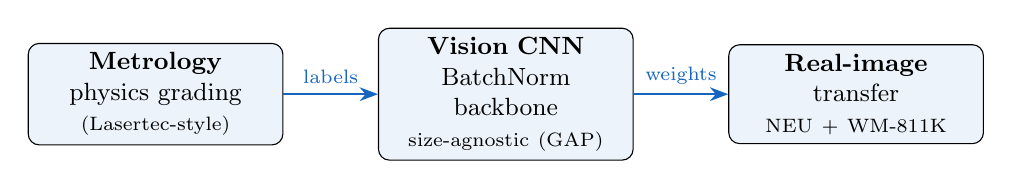
\begin{tikzpicture}[node distance=6mm and 12mm, every node/.style={font=\small},
      box/.style={draw, rounded corners, align=center, fill=discoblue!8,
                  minimum height=11mm, text width=30mm},
      arr/.style={-{Stealth}, thick, discoblue}]
    \node[box] (phys) {\textbf{Metrology}\\ physics grading\\ \scriptsize (Lasertec-style)};
    \node[box, right=of phys] (cnn) {\textbf{Vision CNN}\\ BatchNorm backbone\\ \scriptsize size-agnostic (GAP)};
    \node[box, right=of cnn] (real) {\textbf{Real-image}\\ transfer\\ \scriptsize NEU + WM-811K};
    \draw[arr] (phys) -- node[above]{\scriptsize labels} (cnn);
    \draw[arr] (cnn) -- node[above]{\scriptsize weights} (real);
  \end{tikzpicture}
  \vspace{4mm}
  \begin{itemize}
    \item One CNN backbone (8--16--32 ch, global average pool) serves all tasks.
    \item Multi-metric evaluation throughout: macro-F1, defect-only F1,
          detection recall, false-positive rate --- never accuracy alone.
  \end{itemize}
\end{frame}

% ── 3. Synthetic kerf CNN ────────────────────────────────────────────────────
\begin{frame}{Arm 1 --- kerf quality grading from images}
  \fig[0.62\linewidth]{results/kerf_classifier.png}
  \vspace{-1mm}
  \begin{center}\small
    Synthetic dicing-inspection images, 3 grades.
    CNN \textbf{acc 0.96}, defect-only F1 0.96, reject-recall 0.99.
  \end{center}
\end{frame}

% ── 4. Real images + transfer ────────────────────────────────────────────────
\begin{frame}[shrink=10]{Arm 2 --- real photographs (NEU-CLS) + real-fab transfer}
  \fig[0.50\linewidth]{results/neu_real_classifier.png}
  \vspace{-1mm}
  \begin{center}\small
    \begin{tabular}{lccc}
      \toprule
      Model & accuracy & macro-F1 \\
      \midrule
      RandomForest (pixels) & 0.77 & 0.77 \\
      CNN (cold start) & 0.87 & 0.87 \\
      \textbf{CNN + WM-811K warm start} & \textbf{0.96} & \textbf{0.96} \\
      \bottomrule
    \end{tabular}
  \end{center}
  \begin{center}\small
    Pretraining on 172k real-fab wafer maps transfers to real photos
    (\alert{+9.5 pts}).
  \end{center}
\end{frame}

% ── 5. WM-811K dataset ───────────────────────────────────────────────────────
\begin{frame}{Pretraining source --- WM-811K real-fab wafer maps}
  \fig[0.60\linewidth]{results/wm811k_overview.png}
  \vspace{-1mm}
  \begin{center}\small
    811{,}457 maps / 46{,}293 lots / 172{,}950 labelled. Severe imbalance
    (14.8\% defect); 78.7\% unlabelled --- future self-supervised axis.
  \end{center}
\end{frame}

% ── 6. Metrology -> vision unification ───────────────────────────────────────
\begin{frame}{Unification --- the CNN learns the metrology grader}
  \fig[0.66\linewidth]{results/intelligent_inspection.png}
  \vspace{-1mm}
  \begin{center}\small
    Physics chipping grade $\to$ label; image $\to$ CNN predicts it.
    Agreement \textbf{acc 0.80}, \textbf{reject-recall 0.97}, FPR 0.02.
  \end{center}
\end{frame}

% ── 7. Fusion triage ─────────────────────────────────────────────────────────
\begin{frame}[shrink=10]{Fusion --- fast image triage + physics metrology}
  \fig[0.78\linewidth]{results/inspection_triage.png}
  \vspace{-2mm}
  \begin{center}
    \begin{tabular}{lccc}
      \toprule
      System & fast-path & reject-recall & subsurface-escape \\
      \midrule
      CNN only (image) & 1.00 & 0.93 & \alert{0.07} \\
      \textbf{Fusion ($\tau{=}0.70$)} & \textbf{0.76} & \textbf{1.00} & \textbf{0.00} \\
      Metrology all & 0.00 & 1.00 & 0.00 \\
      \bottomrule
    \end{tabular}
  \end{center}
\end{frame}

% ── 8. Honest scope ──────────────────────────────────────────────────────────
\begin{frame}{Complementary, not redundant}
  \begin{columns}[T]
    \begin{column}{0.5\textwidth}
      \begin{block}{Vision arm sees}
        Chipping --- a surface-visible defect. Fast, every die.
      \end{block}
    \end{column}
    \begin{column}{0.5\textwidth}
      \begin{block}{Metrology arm adds}
        Subsurface crack depth, PL defect density --- invisible to an optical
        image.
      \end{block}
    \end{column}
  \end{columns}
  \vspace{3mm}
  \begin{itemize}
    \item Confidence-gated triage: CNN clears \textbf{76\%} at line speed.
    \item Metrology takes the uncertain \textbf{24\%} and catches the
          crack-only rejects.
    \item \alert{Zero reject escapes at a quarter of the metrology load.}
  \end{itemize}
  \vspace{2mm}
  \begin{center}\small
    Design knows where learned vision helps --- and where physics metrology
    is still required.
  \end{center}
\end{frame}

% ── 9. Summary ───────────────────────────────────────────────────────────────
\begin{frame}{Summary}
  \begin{itemize}
    \item One backbone: synthetic kerf, real photos, wafer maps.
    \item Real-fab pretraining transfers to real images (+9.5 pts $\to$ 0.96).
    \item CNN replicates the optical grader from pixels (reject-recall 0.97).
    \item Fusion triage: metrology-grade safety at line speed for 76\% of dies.
  \end{itemize}
  \vspace{3mm}
  \begin{block}{Reproducible}
    All figures from \texttt{vision/*.py}; multi-metric evaluation; tests guard
    every model. \texttt{github.com/keisuke58/wafer-proc-sim}
  \end{block}
\end{frame}

\end{document}
